\documentclass[a4paper, 10pt, font=plain]{abnt}
\usepackage[utf8]{inputenc}
\usepackage[brazil]{babel}
\usepackage{graphicx}
\usepackage[alf]{abntcite}

\begin{document}
\title{Resumo do livro Agile Coaching}
\author{Hugo Lopes Tavares}
\date{\today}

\maketitle

\part{Coaching Basics}

\chapter{Começando a Jornada}
A missão de um Agile Coach é guiar equipes pra que elas produzam software de qualidade usando métodos ágeis. ``O que um Agile Coach faz?'', ``Como eu faço isso?'', são perguntas que provavelmente desaparecerão ao ler o livro Agile Coaching e esse capítulo cobrirá os tópicos básicos.

\section{O que um Agile Coach faz?}
Seu objetivo é guiar equipes para que elas consigam pensar por si próprias, ao invés de depender de você para ditar leis. Os membros da equipe precisam trocar a maneira como eles pensam e trabalham pra que a implantação de ágil dê certo. Como um agile coach o seu trabalho é guiá-los até que eles encontrem seu próprio caminho.

  \begin{figure}[h]
    \centering
    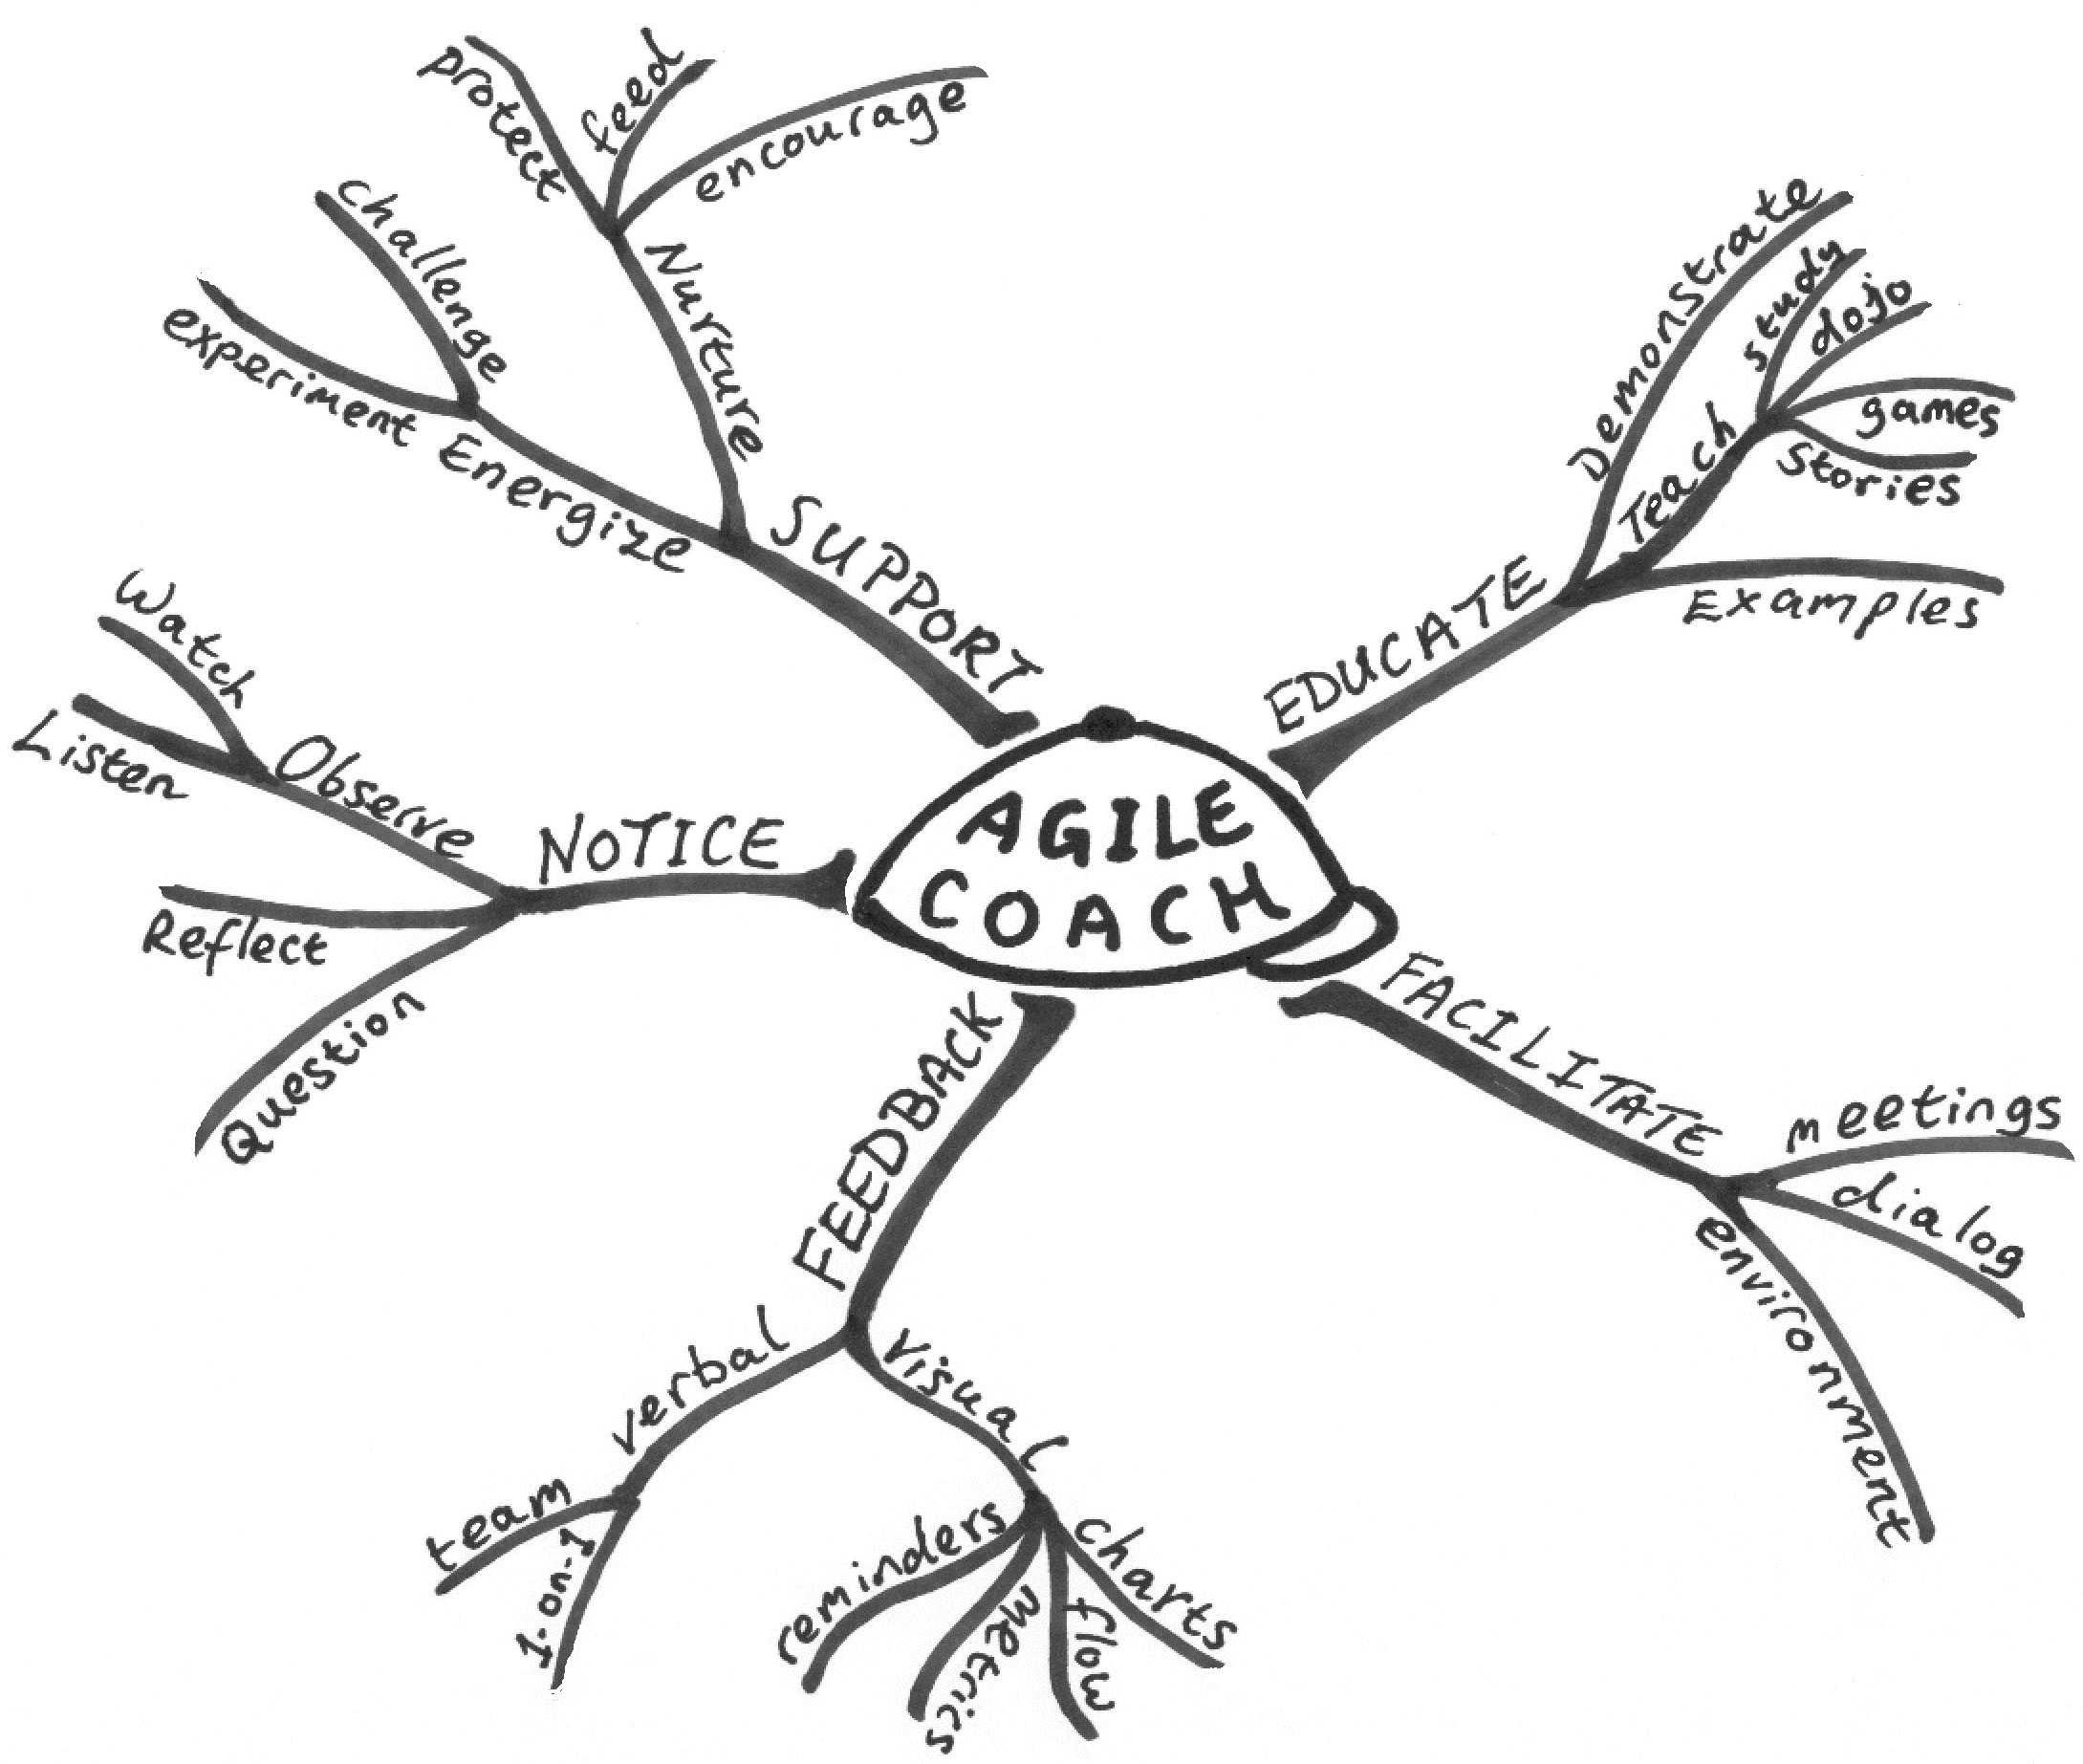
\includegraphics[width=8cm]{mind_map_capitulo1}
    \caption{Mapa mental sobre as tarefas de um agile coach}
  \end{figure}



\section{Desenvolvendo a Atitude de Coach}
O essencial para quem quer se tornar coach é a atitude. Você precisa acreditar que o processo de mudança é possível antes de acontecer e estar sempre aberto a novas idéias.
Algumas das habilidades que todo agile coach precisa desenvolver estão nas próximas seções.

\subsection{Seja um Exemplo}
Todo coach deve dar o exemplo para a equipe. O coach tem que seguir fielmente o que prega, para que possa passar confiança pra equipe. Quando você faz o que fala, as pessoas veêm que podem confiar em você.

\subsection{Mantenha o Equilíbrio}
É normal que as mudanças introduzidas por você causem na equipe uma reação que nem sempre é a esperada. Nunca leve as críticas pro lado pessoal, mantenha-se positivo e firme no papel de coach.

\subsection{Defina um Passo Sustentável}
Não espere perfeição nos primeiros passos de nenhuma equipe, mudanças levam tempo. Paciência é uma das qualidades de um coach.

Se uma equipe está devagar demais pra aplicar o que você tem sugerido, tente achar a causa disso. Será que você está indo rápido demais? Será que não é uma boa hora pra começar?
Seja persistente, afinal, você quer ver resultados. Tente achar novas maneiras pra ajudar a equipe a ver que as mudanças pra Agile são importantes.

\subsection{Pense no seu Vocabulário}
Um coach deve observar o seu vocábulário, pois ele precisa ser claro e você tem que passar idéias facilmente.
Algumas palavras devem ser trocadas para que você possa parecer parte da equipe. Ao invés de dizer ``Você precisa consertar o build'', diga ``Nós precisamos consertar o build''. A diferença é bem pequena, mas os efeitos que essas mudanças causam são importantes, pois mostram que você está do lado da equipe.

Evite criar categorias como ``os desenvolvedores'', ``a gerência'', pois tais categorias criam barreiras na comunicação.

\section{Aprenda com Suas Experiências}
Quando as coisas não sairem como o esperado, não adianta entrar em pânico, pois você deve aprender com os seus erros. Talvez na próxima vez que se deparar com a mesma situção, você deva tentar uma abordagem diferente.

Você não deve ficar encima da equipe o tempo inteiro. Tire um tempo pra refrescar as idéias e se atualizar no que tem acontecido nas comunidades ágeis e fora da empresa. Leia livros, blogs, ouça podcasts e conecte-se com pessoas que tenham os mesmos interesses que você.


\section{Estando Pronto pra Fazer Coach}
Assim como um treinador de esportes, você tem que saber como o jogo funciona. Quando você tiver mais experiência com Agile, poderá usar exemplos reais pra ilustrar seus pontos pra equipes.

Pratique e aprenda como Agile funciona, aprenda a responder perguntas inesperadas. Encontre alguém que queira ouvir e não saiba do que Agile se trata, para que você possa praticar explicações sobre Agile.

Antes de trabalhar com alguma equipe entenda melhor o seu papel. Quais benefícios você traz pra uma equipe? O que a equipe e a gerência esperam de você? Reflita sobre essas questões pra facilitar sua apresentação pra equipe.


\section{Prepare-se pra ser Apresentado}
Começar com o pé direito é muito importante. Você tem que ser apresentado pra equipe, mas trate de fazer isso da melhor maneira. Certifique-se que as pessoas entendam seu papel na equipe.

Ter uma boa apresentação faz com que a equipe tenha credibilidade no seu trabalho. Você precisa fazer com que eles entendam o que você está pronto a oferecer e como você pode dar suporte pra equipe.

A apresentação pode ser feita por várias pessoas dependendo da situação. Você pode ser apresentado pelo empregador, caso você esteja sendo contrato como um coach externo. O empregador pode citar suas qualidades e o que você tem feito como coach ou desenvolvedor.
Caso você já faça parte de uma empresa e tenha sido solicitado pra trabalhar como coach num projeto piloto ou algo parecido, faça com que um gerente que tenha autoridade o suficiente, te apresente pra equipe e mostre a confiança que a empresa tem em você nesse papel. Porém, caso você simplesmente queira disseminar as idéias ágeis, porque você acredita nessa filosofia e tem autoridade pra estender seu papel pra ser um agile coach, não há necessidades de ninguém te apresentar - as pessoas já te conhecem. Junte os membros da equipe e mostre a eles o seu novo papel e responda às perguntas iniciais que aparecerem sobre o movimento ágil.

Após as apresentações gaste um pouco de tempo pra ver como a equipe trabalha - observe de perto. Tente se camuflar como um camaleão para que você consiga pegar os melhores momentos da equipe.

A equipe precisa ter confiança em você antes de começar a seguir suas idéias. Talvez uma sesão pra explicar sobre Agile, algum XP game ou um coding dojo, facilite a introdução dessas novas idéias.



\section{Como começar a fazer coaching}
    \begin{figure}[h]
        \centering
        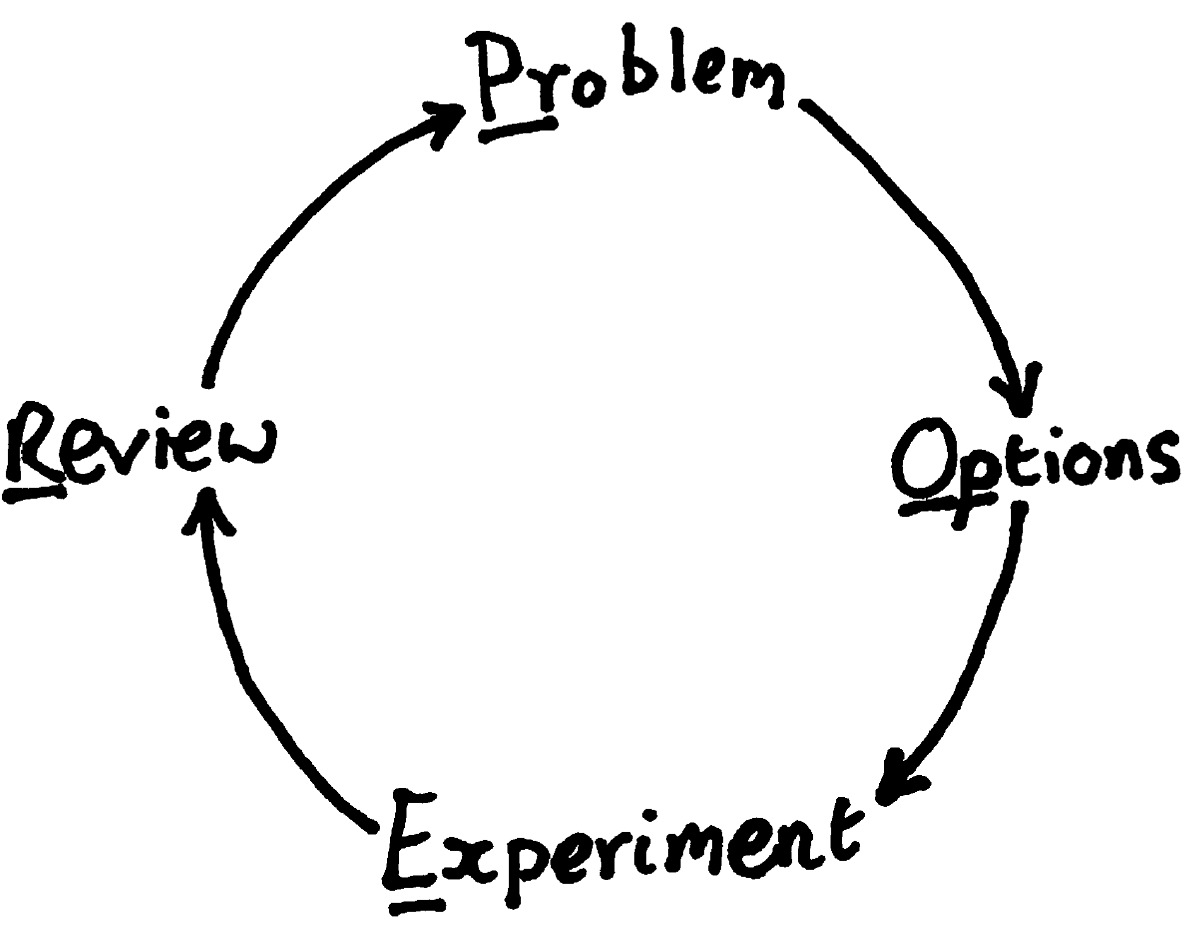
\includegraphics[width=6cm]{PrOpER.png}
        \caption{PrOpER coaching cycle}
    \end{figure}

Não existe lugar certo pra começar. Caso não faça idéia de como começar, faça um brainstorming de idéias para problemas que o projeto tenha. Depois priorize baseado na sua missão como coach - talvez esse seja o lugar pra começar.

O ciclo \textit{PrOpER}, que significa \textit{Problem, Option, Experiment, Review} e está ilustrado na figura acima, pode ser usado pra atacar cada episódio do seu coaching.
Encontre um \textbf{problema} e veja como a equipe trabalha, veja o que precisa ser melhorado. Considere \textbf{opções}, liste pelo menos três opções pro problema. \textbf{Experimente}, pegue uma das opções e tente. \textbf{Revise}, faça uma revisão do resultado. Você melhorou as coisas? Mesmo que não tenha melhorado, você aprendeu algo?


\section{Mantendo o Passo}
Criar equipes ágeis toma tempo e em alguns dias parece não haver progresso. Se as coisas estiverem indo devagar, não se sinta mal. Tente dar um passo a frente a cada dia.
Caso você tenha problemas com os quais não consiga achar soluções, procure outros coaches fora da sua empresa pra poder trocar experiências. Ao invés de imitar outros coaches, tire proveito do estilo de trabalho deles. Veja como eles lidam com determinadas situações e aprenda, e sempre considere integrar alguma das técnicas deles em sua própria abordagem.



\subsection{Calçando suas Botas de Coach}
Para se sentir confortável dando conselhos como um agile coach leva tempo. Se você desempenhava outro papel na empresa e agora é o coach, vai demorar um pouco até que você consiga deixar sua antiga identidade pra trás.
Se você está fortemente envolvido com tarefas do projeto, será difícil encontrar tempo pra guiar a equipe. Quando alguém faz coach ``pelas laterais'', ao invés de ir direto ao ponto, pode focar completamente em melhorar o processo e o trabalho da equipe. Essa posição ajuda a enxergar a imagem inteira para que você possa ajudar a equipe a otimizar o todo.

Como saber se você está indo bem como um agile coach?
\begin{itemize}
  \item Olhando pra trás, a equipe está mais ágil agora do que um mês atrás?
  \item Você teve boas influências na equipe?
\end{itemize}



\subsection{Indo Adiante}
O que acontece com um pepino se ele ficar num recipiente com água salgada? Ele se torna um picles - querendo ou não. Em \textit{The Secrets of Consulting}, Jerry Weinberg alerta para o fato de ``tornar-se'' um picles - se ficamos com a mesma equipe (ou até mesmo empresa) por mais de alguns meses, podemos perder nossa perspectiva. Você pára de notar problemas que eram claros. Você começa a absorver o mesmo comportamento que o resto da empresa e se encontra dizendo, ``Isso é como as coisas são feitas aqui.''

Se você está ciente de que está ``virando um picles'', tente explicar pra alguém de fora como é o processo da equipe e os desafios que você tem encontrado.

Quando tudo estiver indo bem na equipe, provavelmente seu trabalho como coach está finalizado. A equipe já pode se auto-organizar, e ela precisa parar de depender de você pra dar respostas. É hora de ir adiante!


\section{Impedimentos}
Aqui estão alguns impedimentos que você pode encontrar.

\subsection{Não há tempo pra fazer Coach}
Se você está sobrecarregado com as tarefas da empresa e as pessoas confiam a você determinadas tarefas específicas, você não terá como fazer coach. Não desista do papel de coach. Ao invés disso, trace um plano pra que você não seja mais a pessoa na qual tarefas específicas são confiadas.

\subsection{Falta de Experiência}
Quando você se deparar com uma situação que está fora dos seus conhecimentos, fale abertamente com a equipe ao invés de blefar.

Um coach não precisa ter todas as respostas; as vezes é melhor que não tenha. Ajude a equipe a passar por problemas ajudando na discussão e pesquisando o que outras equipes ágeis estão fazendo dentro e fora da sua empresa.

\subsection{Relutantes a Agile}
Há horas em que nos deparamos com sérios impedimentos pra nos tornarmos ágeis. Recomenda-se que você alguns antes de tentar ser coach, pra evitar certas frustações com os envolvidos no processo.

Às vezes os problemas são técnicas, outrora gerenciais. Tenta implantar ágil numa equipe muito crua pode ser problemático - é necessário o conhecimento básico de práticas de desenvovimento de software antes de tentar implantar práticas ágeis.

\section{Checklist}
\begin{itemize}
\item Pratique explicar Agile pra ouras pessoas, pode ser qualquer um que queira ouvir.
\item Faça um pequeno estudo pra encontrar a melhor maneira pra ser apresentado à equipe.
\item Encontre maneiras de mostras que você aplica princípios ágeis com você mesmo - seja o exemplo.
\item Aplique o ciclo PrOpER em suas intervenções.
\item Pause para refletir e aprender com seus erros e faça com que a equipe faça o mesmo.
\item Procure por oportunidades para aprender com outros agile coaches, dentro ou fora da sua empresa
\item Se você trabalhar numa empresa por muito tempo pode acabar se tornando um picles. Quando o tive estiver pronto é hora de ir.
\end{itemize}



\chapter{Trabalhando com Pessoas}
Para ajudar equipes ágeis a melhorarem você precisará ouvir cada membro, um por um, para que você possa ver como as melhorias podem ser feitas. Dê feedback pra equipe ver onde podem melhorar.
Esse capítulo abordará habilidades que ajudam a trabalhar com pessoas numa equipe. Você aprenderá como ouvir as pessoas, como lidar com conflitos e criar acordos.


\section{Ouvindo}
Um coach ouve profundamente. Problemas, angústias, idéias que precisam de ser refinadas. Tente sempre mostrar pra equipe que você está aberto a ouvir o que eles têm a dizer.

Crie espaço pra que as pessoas possam chegar em você e se abrirem, mostre interesse e sempre mostre que você está ouvindo atentamente ao que eles estão dizendo. Quando você ouve com respeito, a pessoa que está falando sabe que você se importa com o que ela diz. Prove que você realmente prestou atenção no que a pessoa falou.

Ouvir atentamente é uma habilidade que você pode aprender. Comece dando total atenção pra quem está falando. Pare tudo que está fazendo e vire-se pra pessoa. Caso a pessoa pareça hesitar em falar abertamente, proponha ir pra algum lugar mais calmo, onde ela se sinta mais à vontade.

Antes de dar qualquer conselho, termine de ouvir. Um grande desafio quando estamos ouvindo alguém é resistir à tentação de começar a aconselhar cedo demais. Foque na pessoa que está falando e tente entender os sentimentos por trás das palavras sem julgamentos.

\subsection{Lendo as Entrelinhas}
As pessoas falam muito mais devagar comparado a velocidade que conseguem pensar, por isso é tão difícil dar total atenção quando alguém está falando. Não perca tempo pensando em respostas quando alguém estiver falando. Preste atenção na maneira como a pessoa está falando, na expressão corporal, como se expressam, no tom de voz, pois assim saberá se a pessoa está com raiva, angustiada, feliz ou desconfortável com alguma coisa, e imagine como ela se sente.

\subsection{Mantendo a Confiança}
No fim da conversa, recapitule os pontos-chaves que você ouviu e cheque-os com a pessoa que vos fala. Você entende suas necessidades?

Não traia a confiança dessa pessoa. Pergunte se ela prefere que o que vocês discutiram é fique entre vocês ou seja exposto pra equipe analisar.

\subsection{``Background Listening''}
Nem sempre você conversará com as pessoas individualmente, você também terá muitas conversas com a equipe inteira. A maioria das regras citadas acima se aplicam pra conversas em grupos.

Se em algum momento você perceber que há alguns pontos citados nas reuniões que são mal-entendidos você pode escolher em fazer uma pausa na reunião e esclarecer pra todos, ou aguardar até o final pra falar. É interessante sempre ter em mãos papel e caneta pra anotar observações durante a reunião.

\subsection{Dando Feedback}
Quando você observa que algum comportamento não está funcionando pra equipe ou pra algum membro em especial, você naturalmente terá vontade de ajudá-los a ter melhorias. Você precisa compartilhar suas observações, pra que de alguma forma você possa influenciar as pessoas pra que mudem suas atitudes e comportamentos.

Seu primeiro passo pra dar feedback é separar suas informações básicas (o que você viu ou ouviu) de suas avaliações e sentimentos sobre a situação. Fale sobre os acontecimentos da sua perspectiva e dê exemplos específicos do que você viu e ouviu ao invés de interpretações. O quanto mais cedo você disser, melhor, pois é mais fácil pra pessoa falar do que fez e o motivo o quanto mais cedo.

Depois disso é a vez das outras pessoas. Ouça a suas experiências dos acontecimentos. Talvez exista um bom motivo que explique suas ações e você não saiba.

Caso você veja que ainda é posível fazer mais melhorias, dê sugestões de como eles devem lidar com tais situações no futuro. Peça idéias, também, assim você pode mostrar os prós e contras de cada opção.


\section{Resolvendo Conflitos}
Como coach você pode se ver em situações em que a equipe está presa por confrontos internos. Se você perceber que há conflitos internos na equipe, tire um tempo pra ouvir cada indivíduo.

Antes de agir como um pacificador, veja se o conflito não pode ser resolvido sem sua ajuda. O motivo disso é que se você intervir em cada conflito que surgir, sempre alguém virá choramingar com você, como se fosse um pai chamado pra resolver conflitos entre crianças.

Sempre que você estiver agindo como um mediador, lembre-se que você não pode tomar lados. Ouço cada lado da discussão e mostre que você entende o que está sendo dito, recomeçando a explicação do problema com suas próprias palavras. Explique os fatores que você vê na situação e talvez seja útil estudar as forças envolvidas.

Lembre-se que diferença em opiniões é algo saudável. Muita ênfase em paz e harmonia pode sinalizar que a equipe está sendo complacente. Sempre que for tomar decisões importantes, lembre-se de certificar que você considerou opiniões diferentes.



\section{Criando Acordos}
Quando você introduz novas práticas, é bom saber se todos concordaram com as idéias. Existem equipes em que nem todos compram a idéia da mudança, alguns membros ainda continuam céticos. Uma técnica que ajuda a diferenças de opiniões é a ``gradientes of agreement''.

Ao invés de perguntar esperando por um voto de sim ou não, você cria uma escala, onde os extremos são Endossar e Bloquear.

\begin{figure}[h]
    \centering
    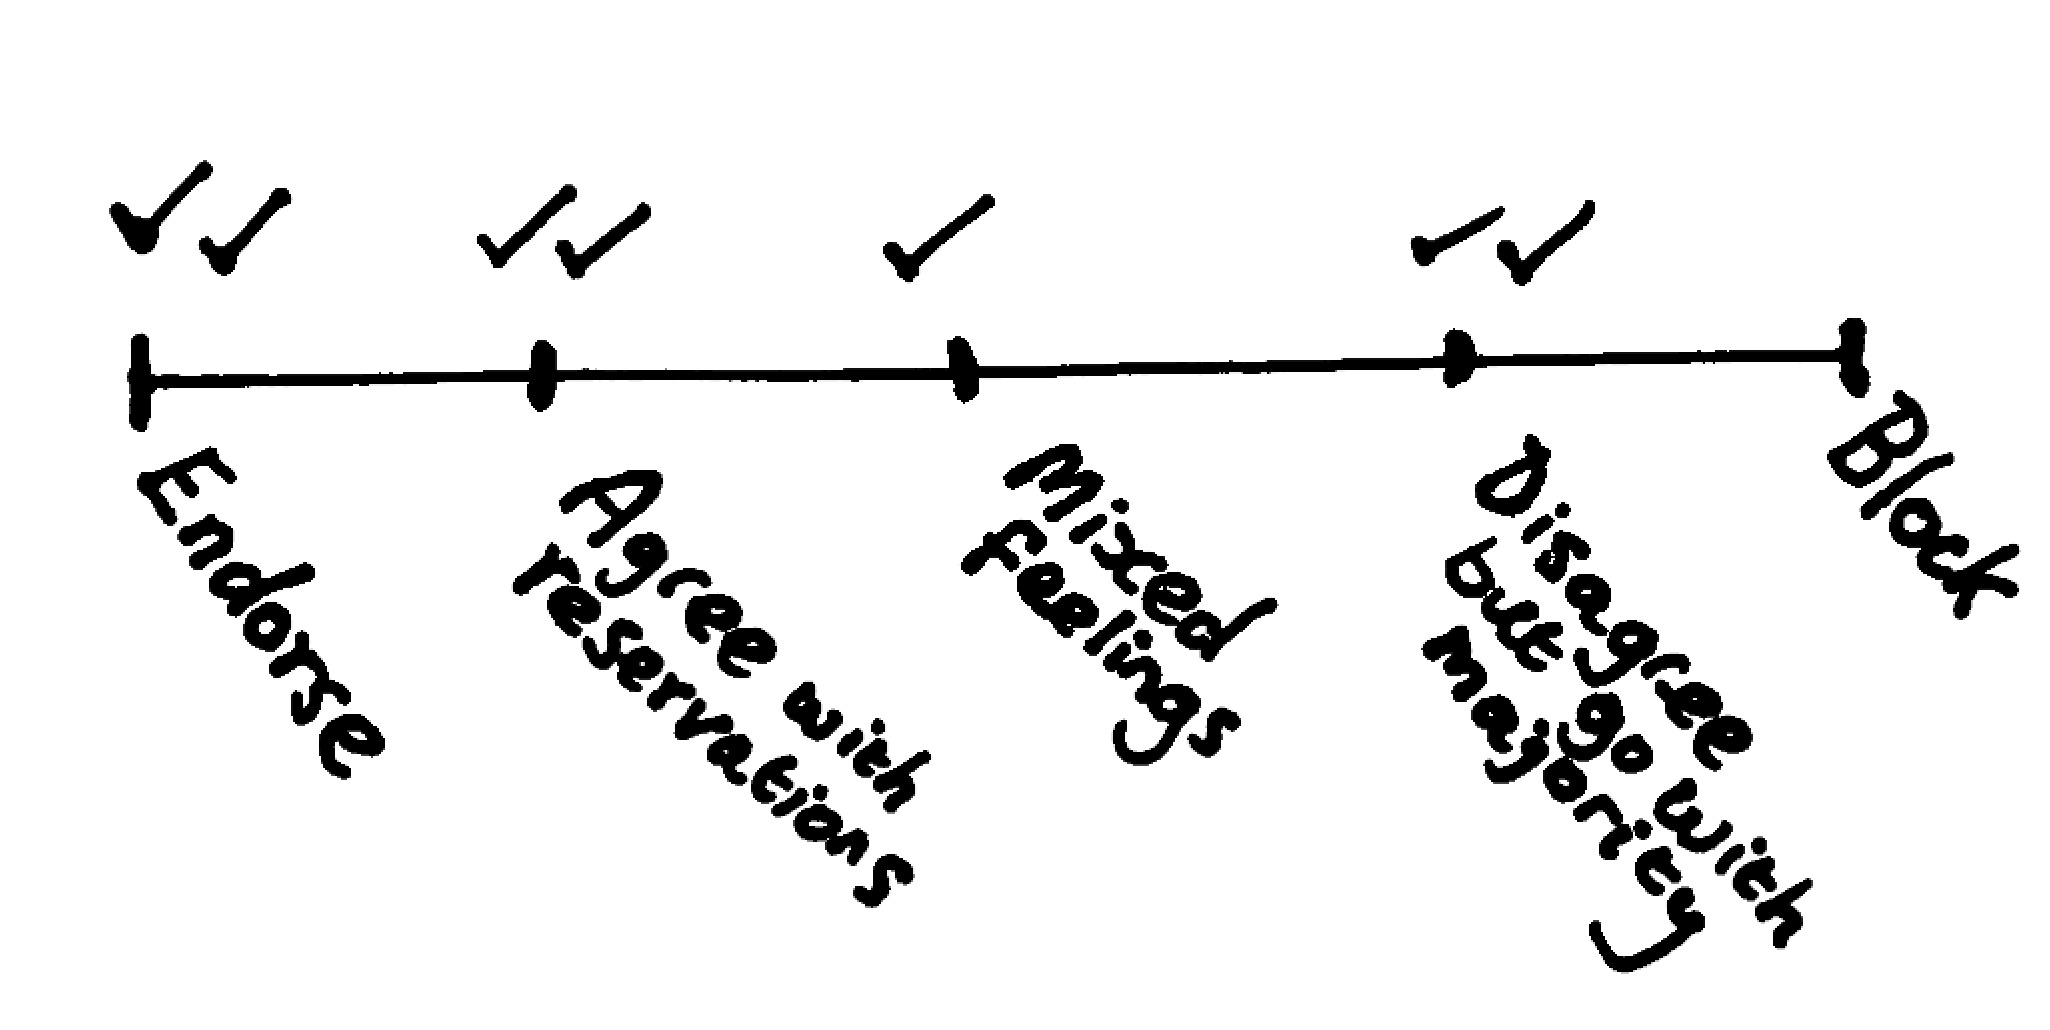
\includegraphics[width=8cm]{gradient_scale}
    \caption{Um exemplo de ``gradient scale''}
\end{figure}

Usar uma escala dessas possibilida descobrir se há alguma falta de consenso. O consenso é importante porque se alguma pessoa não concorda com alguma ação, ela não a implementará entusiasticamente.

A técnica ``gradient scale'' pode ser usada pra estabelecer níveis de concordância entre a equipe. Caso não seja possível usar desenhos da escala, votar em opções de zero a cinco com os dedos da mão também pode ser útil. Independente do método que você escolher, leve-o a sério e pesquise sobre suas preocupações.

\section{Impedimentos}
A seguir estão alguns impedimentos que você pode encontrar.

\subsection{Explosão Emocional numa Reunião}
Caso haja alguma explosão emocional numa reunião, é recomendável que você dê um tempo à pessoa pra que ela recupere sua compostura. Antes de retomar a reunião converse com essa pessoa e entenda seus motivos. Veja se a equipe prefere continuar a reunião ou resolver o problema que causou tal excitação primeiro.

\subsection{Falta de Habilidade das Pessoas}
Algumas pessoas acham que entrando na carreira de desenvolvimento de software não precisarão lidar com pessoas, porque acham isso difícil. Você deve tomar cuidado, pois cada pessoa tem suas preferências em como comunicar-se. Talvez você tenha que ser mais direto com certas pessoas e dar mais espaço a outras.

\subsection{Diferenças Culturais}
Há significados diferentes pra várias coisas em culturas diferentes. Em certas culturas um "sim" significa "Sim, estou escutando" e não um "Sim, eu sei como fazer isso."

Ajude sua equipe a ficar mais antenada com diferenças culturais, tais como tolerância em ambiguidade e individualismo. Uma maneira de fazer isso é estudando o trabalho de Geert Hofstede em dimensões culturais com a equipe\footnote{http://www.geert-hofstede.com/}.

\section{Checklist}
\begin{itemize}
\item Acostume-se a ouvir profundamente pra entender os problemas que aparecem e pra criar confiança. Dê completa atenção às pessoas enquanto conversam e peça esclarecimentos pra ver se você realmente entendeu o que disseram
\item Quando estiver dando feedback, separe o que você viu ou ouviur dos seus sentimentos sobre a situação. Dê exemplos específicos do que você notou, ao invés de comentários. Diga o que você viu ou iuviu, e depois peça explicação dos acontecimentos. Agora junte todos pra ter idéias de como lidar com a mesma situação numa próxima vez.
\item Se um conflito surgir, tenha certeza que todos os lados compartilham seus pontos de vista. Não resolva todos conflitos, senão vão confiar a você o papel de pacificador ao invés de aprender com o tempo.
\item Use ``gradients of agreement'' pra descobrir o nível de aceitação de uma mudança. Isso permite que a equipe discubra se existe mais ou menos discordâncias.
\end{itemize}


\chapter{Liderando Mudança}
Às vezes você estará introduzindo novas práticas ágeis, outras vezes ajudando a equipe a refinar seu processo. De qualquer forma, você precisa guiar o time pelas mudanças.

Comece devagar; dê a equipe um tempo pra refletirem sobre as mudanças antes de pressioná-los e procure oportunidades pra que a equipe aprenda mais sobre agile.

\section{Apresentando a Mudança}
Quando você começar a defender técnias ágeis pra uma equipe, perceberá que algumas pessoas terão objeções. É natural as pessoas querem entender melhor os riscos mesmo que tenham um motivo convincente. Conte histórias sobre equipes que obtiveram sucesso com Agile e mostre o que é possível fazer com tais técnicas.

Mostre que você tem confiança na equipe, eles precisam acreditar que você crê neles pra obterem sucesso e encorajá-los a tomar o primeiro passo.

Tome cuidado pra não inserir muitas mudanças de uma vez só. Deixe novas idéias aparecerem. É preciso dar tempo à equipe pra conversar e refletir sobre como implementar tais mudanças e nas implicações que poderão surgir e em como eles encararão isso.


\subsection{Mostre-os Como}
Somente convencer de que a mudança é necessário não é o suficiente pra fazer com que a equipe mude; você precisa mostrá-los como começar. Organize treinamento pra equipe; demonstre como realizar determinadas tarefas sentando junto, explicando; deixe visível o progresso da equipe.


\subsection{Apresente o Problema}
Como coach, você verá muitas oportunidades pra introduzir melhorias. Porém, antes de compartilhar suas idéias, esteja preparado pra apresentar o problema que está conduzindo a mudança. Deixe claro as implicações que haverão caso a equipe não faça as mudanças necessárias.

Nunca seja grosseiro, pois pode fazer com que o problema pareça difícil demais pra ser superado. Um de seus objetivos é deixar claro os motivos que podem surgir caso a mudança não seja feita. Tome cuidados extras pra não criticar a maneira com qual a equipe trabalha. Seu foco são as melhorias no processo, não em performances individuais.


\subsection{Crie Propriedade para Mudança}
Uma vez que os problemas foram apresentados, é hora de focar em soluções. Encorage os membros da equipe a olhar em resultados positivos pra melhor seu processo ágil. Crie uma propriedade coletiva conversando sobre pros e contras de fazer mudanças.

Deixe que eles saibam as opções que você vê e os convide pra dar novas idéias. Essas conversas se tornam uma parte da vida da equipe uma vez que eles começam a fazer retrospectivas. Uma abordagem em adotar Agile é fazer com que retrospectivas sejam a primeira prática a ser realizada. Retrospectivas provêem a equipe uma série de pontos a serem discutidos e mudanças a serem acrescentadas em poucas semanas.


\subsection{Faça da Mudança um Experimento}
Quando encontrar alguma resistência, proponha tentar algo diferente como um experimento. Encarar uma mudança como um experimento faz com que a equipe foque no benefício, uma vez que a equipe precisa avaliar se o experimento obteve sucesso.

Uma vez que a equipe decide e tenta uma mudança como um experimento, os membros acostumam-se com a nova maneira de trabalhar. Depois disso, voltar pra maneira antiga de trabalho é uma mudança que a equipe hesitará em fazer. Comece com mudanças pequenas, pra que a equipe se preparare para as maiores.

\section{Faça Perguntas}
Outra maneira de liderar uma equipe é fazendo perguntas. Quando você faz uma pergunta a alguém, você demonstra respeito e interesse em sua opinião. Eles precisam forçar o cérebro a pensar numa resposta, e quando fazem isso, caem na sua indagação de melhoria na forma como a equipe trabalha. Uma pergunta provocativa pode até mesmo fazer com que sigam com sua conversa e tomem alguma ação.

Muitas vezes as pessoas se prendem a crenças que acreditam ser verdadeiras. Você pode usar perguntas pra desafiar suas crenças sobre como a empresa trabalha e sobre o que eles podem ou não fazer.

Não faça perguntas que possam ser respondidas com "sim" ou "não". Faça perguntas que dêem margem à conversa, perguntas como "Como fazer isso?", "O que aconteceria?"; perguntas como estas fazem com que a pessoa reflita e compartilhe suas opiniões.

Cuidado com com perguntas que tenham "Por quê?", pois podem parecer críticas a idéias ou acusações. Por quês tendem a tratar de problemas, e não de soluções.

\subsection{O que Perguntar}
Existem vários tipos de perguntas, a seguir há algumas interessantes.

\subsubsection{Peça Ajuda}
Peça ajuda a alguém de uma forma mais pessoal, evite fazer isso em reuniões. Mostre algum problema com o qual você está lidando e peça ajuda. A pessoa pode oferecer idéias, suporte ou até mesmo algo mais prático. A maioria das pessoas ama ajudar e se sentirão lisonjeados em te ajudar.

\subsubsection{Perguntas Intrigantes}
Você pode facilitar o raciocínio de alguém fazendo perguntas intrigantes. Tais perguntas forçam a pessoa a desfocar dos detalhes do problema e olhar para o problema de uma perspectiva diferente.

\subsubsection{Perguntas que Fazem Refletir}
Incentive a equipe a notar mais em como eles trabalham, fazendo perguntas sobre o que eles notaram mais a frente. Compartilhe suas observações pra ajudá-los a entender o seu interesse. Pegue experiências do dia-a-dia, as observações dos membros da equipe e procurem por melhorias baseado no que foi bom ou ruim.

\subsubsection{Cinco Por Quês}
A técnica dos Cinco Por Quês \textit{(Five Whys)} foi inventada por Taiichi Ohno, que pode ser usada pra achar a raiz de algum problema. A técnica consiste em pegar um problema da superfície, depois perguntar o que causou tal problema, o que causou o outro, e o outro, e o outro e o outro. Quando você tiver perguntado "Por quê" cinco vezes, achará o problema real, que será um problema sistemático. É importante explicar pra equipe a técnica, pra não parecer que os por quês estão sendo repetidos por descontentamento com a resposta.


\subsection{Quando Não Fazer Perguntas}
Cuidado para não fazer perguntas quando for orientar alguém da equipe. Se você fizer alguma pergunta, terá que aceitar a resposta e se você discordar, será mais difícil dar o conselho que você queria.

Se você só faz perguntas, deveria compartilhar mais o que você sabe, senão as pessoas não se abrirão pra você. Tenha em mente que se você não se importa com a resposta, quando você fizer alguma pergunta, poderá parecer que está tentando apontar falhas em alguém.

Quando existe pouca confiança entre você e alguém na equipe. Certamente essa pessoa reagirá defensivamente e a resposta não será verdadeira. Ao invés de perguntas, nesses casos é melhor uma conversa aberta e direta.


\section{Apoie o Aprendizado}
Sua equipe precisa aprender sobre Agile antes de adotar práticas ágeis. Encoraje-os pra que se dediquem a estudar um pouco sobre agile, seja no tempo de trabalho ou em casa. Faça com que eles tomem a iniciativa pra aprenderem por si próprios ao invés de dependerem de você como fonte de conhecimento sobre Agile.


\subsection{Crie Oportunidades de Aprendizado}
As idéias ágeis ainda em expansão, estão evoluindo, assim, você precisa estar sempre atualizado sobre o que está acontecendo ao redor do movimento ágil. Existem várias maneiras de aprender sobre Agile, e uma de suas funções é tornar isso fácil.

Uma maneira poderosa de apresentar idéias sobre Agile é organizando apresentações com membros da própria empresa, pra falarem sobre suas experiências com Agile. É uma maneira de criar oportunidades pra que amigos de trabalho possam mostrar o que aprenderam sobre Agile, além de dar oportunidades de falarem em público.

Você pode também convidar pessoas de fora, experts da área ou conhecidos de grupos locais sobre agile, pra compartilharem com você e sua equipe experiências de como usaram ou usam Agile em algum projeto ou empresa.


\subsection{Indo Para Fora da Empresa Para Aprender}
Conferências são uma ótima maneira de expôr a equipe a novas idéias, porque lá haverá pessoas com mesmos problemas, pessoas que compartilham experiências e é possível encontrar ajuda. Inclusive é uma maneira de abrir os olhos de quem está na empresa por muito tempo.

Sua equipe pode também encontrar ajuda e encontrar novas idéias em grupos locais sobre agile. Ao invés de informá-los sobre o próximo encontro que você irá, convide-os pra ir com você.


\subsection{Facilitando Reuniões}
Sempre que uma nova mudança estiver pra ser feita, mostre a equipe como se faz. Na primeira vez que uma equipe ágil fizer uma reunião, seja uma retrospectiva ou uma reunião de planejamento, ofereça-se pra facilitar a reunião, pra mostrá-los como é feito. Durante a reunião explique como o processo funciona, pra que na próxima vez eles possam fazer sozinhos. Da próxima vez, planeje junto da pessoa que será o facilitador da reunião e durante a reunião, não interrompa até que a reunião termine - a não ser que comece a sair do foco.

Após a reunião, exponha suas idéias do processo e pra ser melhor ainda na próxima vez, peça feedback da equipe.

Pra tornar a reunião eficaz, você precisa:
\begin{itemize}
\item escolher um horário que seja adequado a todos da equipe
\item arrumar um lugar adequado pra fazer a reunião
\item manter sempre o foco da reunião
\item manter a reunião fluindo, tornando-a fácil para as pessoas
\item encoraje todos a participar com idéias, opiniões, dúvidas ou respostas
\item resuma os pontos principais pra ter certeza que tudo foi bem compreendido
\item termine a reunião tendo certeza que o que foi gerado na reunião tenha sido devidamente gravado
\end{itemize}


\section{Impedimentos}

\subsection{Algumas Pessoas Nunca Mudam}
Algumas pessoas gostam de ser as primeiras a acolher a mudança, outras preferem ser as últimas. Não se prenda a essas pessoas, elas gostam de ser as últimas. Quando Agile for o padrão, tenha certeza que elas adotarão.


\subsection{Dando de Cara com as Políticas da Empresa}
Quando a mudança começa a ser feita, você irá dar de cara com políticas internas da empresa. Algumas pessoas - gerentes de projeto, arquitetos - podem achar que seu trabalho está em perigo. Procure mal-entendidos e tente resolvê-los.

Um líder técnico pode ser um impecílio na mudança da equipe pra Agile e se você é muito crítico sobre essa pessoa. Invista algum tempo entendendo a perspectiva da pessoa, só assim você irá conseguir argumentos pra convencê-lo com seus planos sobre da mudança.


\subsection{Planos de Trabalhos Conflitantes}
Às vezes é difícil manter o foco quando outras pessoas estão esperando que você resolva seus problemas. Por exemplo, alguém veio reclamar sobre não poder colar nada na parede. Você pode concordar que é um problema, mas talvez não seja a hora certa pra resolver isto.

Tente ser neutro em público e explique em particular sobre o que você tem feito pra tentar resolver os problemas, evitando ficar com reputação de pessoa negativa. Explique os problemas nos quais você tem no momento e peça que a pessoa te ajude. Depois você pode se esforçar pra resolver os problemas ou concordar que realmente não é uma boa hora.


\section{Checklist}
\begin{itemize}
\item Converse sobre agile, demonstre, ofereça-se pra ajudar as pessoas; encoraje e inspire a equipe, mostrando que Agile pode funcionar
\item Apresente o problema pra equipe; ajude-os a enxergar o motivo da mudança; converse individualmente com os membros da equipe
\item Quando deparar com resistência, tente entender de onde vem. Veja se foi a forma com a qual alguma idéia foi apresentada, se existem bons motivos pras pessoas se preocuparem com a idéia, veja se as observações procedem
\item Faça perguntas pra forçar a equipe a melhorar seu processo ágil. Peça ajuda, faça perguntas intrigantes, perguntas que façam as pessoas refletirem, use a técnica dos "Cinco Porquês"
\item Apoie novas maneiras de aprender sobre agile: livros, blogs, podcasts. Organize apresentações, grupos de estudo. Deixe-os informados sobre eventos sobre Agile e leve-os pra grupos locais sobre Agile
\item Faça com que novas reuniões sejam fáceis, sendo o facilitador na primeira vez. Exponha suas idéias sobre o processo da reunião. Ajude a equipe a preparar a próxima reunião, e depois dê a eles feedback
\end{itemize}




\chapter{Montando Uma Equipe Ágil}
Equipes ágeis não aparecem do nada, leva tempo pra equipe ser formada. Quando uma equipe não se une, as pessoas ficam frustadas e o software que eles produzem reflete isso.

Você pode ajudar uma equipe a ser mais unida fazendo com que os membros se conheçam melhor, melhorando o ambiente de trabalho. Procure maneiras pra ajudar a equipe inteira saber aonde o projeto está indo.

\section{Ajudando uma Equipe a se Unir}

\subsection{O Lado Social}
Fazer com que uma equipe seja unida e que os membros confiem uns nos outros, leva tempo. Trabalhando junto a equipe começa a entender as perspectivas e problemas uns dos outros. Encontros, em especial o Daily Standup (ou Standup Meeting) e retrospectivas, são uma oportunidade pra equipe se conhecer melhor.

Você deve criar oportunidades pra equipe se conhecer melhor, seja trocando histórias pessoais ou saindo junto.

\subsection{Crie Confiança}
Colaboração em equipe cria confiança. Você pode guiar a equipe a criar confiança uns nos outros mostrando que é seguro se abrir. Seja transparentes sobre motivos, exponha informações sobre experiência, sentimentos e opiniões - isso faz com que as pessoas se abram também. Admita quando você errar. Peça ajuda regularmente.

Caso exista no ambiente de trabalho alguma cultura de punição ou críticas a erros, isso faz com que as pessoas não se sintam segura. Os membros da equipe precisam se sentir confortáveis pra dizer quando precisam de ajuda, e quando isso acontecer eles se sentirão felizes em compartilhar conselhos e ajudar os amigos de equipe.

Se as pessoas se sentirem inseguras - se estiverem com medo de serem demitidas, por exemplo - você não conseguirá fazer nenhum agile coaching. Nesse caso, você precisa dar suporte à equipe da maneira que puder até que a situação se resolva.


\subsection{Preenchendo a Lacuna}
Criar confiança entre pessoas com papéis diferentes é mais difícil do que entre pessoas com o mesmo papel. Você pode sugerir que as pessoas troquem de papel por um perído curto de tempo, pra verem como é o trabalho da outra pessoa. Um desenvolvedor poderia ficar por uma semana como testador, por exemplo (caso possua os conhecimentos necessários) ou parear com um testador contribuindo com o máximo possível.

Às vezes por não entenderem direito o trabalho do outro as pessoas assumem que o seu próprio trabalho é mais difícil. Sem respeito mútuo uma equipe não será bem sucedida. Você pode demonstrar respeito pelas pessoas pedindo opiniões ou ajuda e levando seus interesses e idéias a sério. Outros notarão e imitarão você.

Se uma pessoa parece estar infeliz com outra, a convide pra um café e discuta isso. Quais suposições que a fizeram isso acontecer? Quais explicações possíveis existem pra isso?


\section{Criando um Ambiente Para a Equipe}
Uma equipe precisa de um ambiente de trabalho compartilhado pra fazer com que a informação flua. O ideal é que toda a equipe trabalhe na mesma sala. Uma área pequena perto da equipe, onde eles possam tomar um café ou conversar, melhora o entrosamento da equipe. Uma sala de reuniões próxima é útil por questões de privacidade e pra discussões que não atrapalhem a equipe. Esse passo é crucial pra fazer uma equipe ágil dar certo. Todos devem trabalhar na mesma sala, sempre.

Se algumas pessoas forem relutantes a esta idéia, encoraje-os a personalizar seu lugar de trabalho, seja com livros, plantas ou fotos, pra que elas se sintam à vontande pra trabalhar.

Vale lembrar que não é só o espaço físico com o qual você deve se preocupar. O ambiente virtual também deve ser levado em conta. Encoraje a equipe a ter uma wiki ou repositórios de documentos compartilhados. Eles também precisam estar a par do setup do ambiente de desenvolvimento e de testes.


\section{Equilibrando Papéis}
A relação entre clientes e desenvolvedores é crucial, porque eles precisam trabalhar juntos pra criar o melhor produto. Todos precisam se sentir parte da mesma equipe, trabalhando com o mesmo objetivo final. Deixe claro as responsabilidades de cada papél pra equipe inteira.

O cliente (\textit{customer}, ou \textit{product owner} no Scrum) é a pessoa responsável por priorizar o que o software deve fazer. A equipe de desenvolvimento é responsável por decidir como criar o software e por comunicar ao cliente o tempo que levará. O cliente pode definir datas pra que o software seja entregue, mas não pode tornar o escopo fixo - o escopo é definido em equipe.

Normalmente o cliente é um gerente de produtos (\textit{product manager}) que trabalha com vários usuários e \textit{stakeholders} (clientes reais, as pessoas que pagam pelo software) pra decidir o que o software deve fazer. Em desenvolvimentos grandes, o papel de cliente pode ser demais pra uma pessoa só, e assim é formada uma equipe com a expertise necessária pra lidar com user stories e priorizá-las, que representará o cliente - analistas de negócio, representantes do usuário ou designers de interação, dependerá do projeto.

Às vezes a melhor solução é um "cliente-perto" (\textit{near-customer}), que ajuda a trabalhar nos detalhesdos requisitos com a equipe, e um "cliente-longe" (\textit{far-customer}) que toma decisões sobre as prioridades do negócio. O cliente-perto pode ser um analista de negócios que fica perto da equipe, enquanto o cliente-longe pode ser um gerente de produtos que fica perto das operações do negócio e das equipes de marketing.

Se os papéis saem do equilíbrio, um dos lados terá trabalho em excesso. Se o excesso estiver do lado do cliente , os desenvolvedores não terão tempo suficiente e terão que adivinhar o que o cliente quer. Se não houver desenvolvedores o suficiente ou estão trabalhando mais devagar do que o esperado, a parte de negócio estará desapontada com os resultados. Como coach você pode ajudar fazendo com que os efeitos colatereais do desequilíbrio sejam mais visíveis, para que a gerência possa pensar em como resolver tais problemas.



\section{Energizando a Equipe}
A seguir estão algumas idéias de como energizar a equipe e ajudá-los a encontrar sua própria motivação.


\subsection{Nem Tão Fácil, Nem Tão Difícil}
Todo mundo precisa ser suficientemente desafiado, nem entediado, nem ansioso. Essa é a parte do trabalho que as pessoas mais gostam.

Se for muito fácil, os desenvolvedores ficarão entediados e desmotivados. Se houver muitas coisas fáceis a serem feitas, encoraje-os a automatizar.

Às vezes o trabalho parece impossível de ser feito e as pessoas acabam travando no problema. Quando isso acontecer, é necessário dividir em partes mais gerenciáveis, para que a equipe consiga pegar alguma parte pra começar o trabalho.

Sustente uma cultura onde não há problemas em experimentar e aprender sobre um problema que a equipe precisa resolver. Às vezes a equipe pode achar que perdeu tempo com experimentos, mas é uma maneira rápida de aprender e barata de avaliar os custos da decisão errada.


\subsection{Encontre um Objetivo Atrativo}
Saber que o que a equipe está produzindo um produto que é útil ajuda a equipe a se empenhar. Se possível, arranje um encontro entre a equipe e usuários finais. As necessidades dos usuários serão mais vivas pra equipe e darão idéias de como eles podem ajudar a fazer um produto melhor.

Equipes ágeis planejam e modelam seu próprio trabalho. Uma vez que a equipe entender que eles não precisa esperar por permissões, pode deixá-los livres pra um começo.


\subsection{Tempo pra Inovação}
Quando membros de uma equipe ágil trabalham sem parar num fluxo contínuo de user stories, pode acabar prejudicando a equipe.

Se as pessoas não tiverem tempo pra explorar ou aprender alguma coisa nova, elas podem se sentir desmotivadas. Deixe um tempo no planejamento da iteração pra equipe explorar novas idéias.

Quando os membros da equipe tem tempo pra buscar por inovação, eles ficam mais felizes no trabalho. Isso melhora a energia da equipe e remove atritos de tarefas relacionadas ao projeto. Incentive a inovação dentro da equipe, deixando tempo reservado pra cada um. Use de técnicas como \textit{Gold Cards}\footnote{veja ``Innovation and Sustainability with Gold Cards'' apresentado na XP Universe 2001 Conference} pra que cada membro sinta-se a vontade pra ficar um dia por conta de aprender alguma coisa nova e no fim da iteração compartilhar o que aprendeu.


\subsection{Celebre o Sucesso}
Encontre maneiras de celebrar o sucesso a cada release. Saia com a equipe pra almoçar, beber ou até mesmo comer uma pizza. A comemoração aumenta os laços da equipe.

Ajude a equipe a mostrar pra pessoas de fora seu sucessso. Faça apresentações de demonstração, mande convites pra pessoas de fora. Uma palavra de obrigado dos clientes é sempre bem vinda e aumenta o moral da equipe.


\subsection{Não Desmotive}
As pessoas começam motivadas. Se nada as desmotivar, elas tendem a continuar motivadas! O que faz as pessoas continuarem motivadas é o que elas fazem. E o que faz as pessoas ficarem desmotivadas é a situação com que elas trabalham - incluindo estresse e cultura da empresa.

Computadores rápidos, um café decente, um bom salário, não seriam notados se estivessem lá. Porém, a falta deles poderia desmotivar os membros da equipe. Como coach você talvez não possa influenciar diretamente nisso, mas vale a pena conversar com a equipe pra ver o que os incomoda. Você pode encontrar coisas fáceis de resolver, como melhorar o ambiente de trabalho.


\subsection{Cuidado Com Os Incentivos}
Tenha cuida ao usar "incentivos" pra motivar pessoas. Esquemas de incentivos pessoais podem atrapalhar o trabalho em equipe, pois ajudar os colegas de trabalho não faz sentido se todos estão concorrendo a um bônus.

Caso um bônus seja oferecido pra equipe quando uma tarefa for terminada, nada mais nada menos do que o que for preciso fazer pra ganhar o bonus será feito. Se a gerência tem um esquema de bônus, converse com eles pra que esse bônus não tenha como foco indivíduos isolados, mas a equipe como um todo. A equipe produzirá mais e fará um produto melhor quando estiverem motivados.



\section{Impedimentos}

\subsection{Equipes Não São Especialistas-Generalista \textit{Cross-Functional}}
Algumas empresas organizam equipes por disciplinas, como testadores, desenvolvedores, analistas, designers e etc. Isso é um grande bloqueador na transição pra Agile, porque um dos princípios ágeis é equipes especialistas-generalistas \textit{crosss-functional}, com diferentes disciplinas, que desenvolvem junto o melhor software possível.


\subsection{Não Há Cliente Presente}
Às vezes a equipe de desenvolvimento está num lugar e o cliente em outro. Se não manejado bem, o cliente remoto pode ser um grande problema na comunicação da equipe.

Criar uma boa comunicação com o cliente remoto nesse caso, é vital. Encoraje o cliente a se encontrar pessoalmente com a equipe, pra que todos possam se conhecer. Isso pode ser feito na primeira reunião de planejamento. Depois disso você pode encorajar conversas por telefone ou chat na internet, de preferência com webcam - pra que todos possam se ver e criar um clima mais amigável.


\subsection{A Equipe É Grande Demais}
Se você está trabalhando com uma equipe com mais de dez pessoas, está propício a ter problemas na comunicação e responsabilidade dentro da equipe. Qualquer reunião se torna mais longa, e os membros se sentem menos motivados por parecem pouco dentro da equipe. Trabalhe com a equipe pra dividir em subequipes - idealmente equipes centradas nas funcionalidades do cliente (\textit{feature teams})\footnote{veja Scaling Lean \& Agile Development, 2009}.


\subsection{A Equipe É Um Conjunto de Recursos}
Agile não funciona bem quando um conjunto de pessoas trabalhando em vários projetos tenta aplicar Agile como se fossem uma equipe só. Agile assume um projeto por vez. Quando a equipe trabalha em vários projeots, não há grandes objetivos que são atrativos. Você notará que prioridades em diferentes projetos mudam, e isso causa interrupções que deveriam ser trabalhadas dentro da equipe. Recomenda-se não aplicar Agile nessa situação.



\subsection{Os Membros da Equipe Isolam Alguém da Equipe}
Você pode notar que a equipe está evitando trabalhar com uma determinada pessoa. Será que é um problema de falta de confiança? Ou seria um problema prático? Talvez porque a pesssoa não tomou banho de manhã?

Tente conversar com a equipe (quando a pessoa isolada não estiver por perto) pra ver qual é o motivo do isolamento. Depois converse com a pessoa em questão, veja se ela está sabendo da situação. Envolva o departamento de Recursos Humanos caso você perceba que a pessoa está distraída por questões de doença, estresse ou depressão.

\subsection{Team Becomes Complacent}
Teams often become insular when there is a lack of exposure to other
teams and business goals. If you become concerned about the team
being too complacent, it may be worth trying to increase the visibility
of the team’s work to senior stakeholders and increase the feedback to
the team about business value generated by their work.



\section{Checklist}

\begin{itemize}
\item Crie oportunidades pros membros da equipe se conhecerem melhor, o que a ajuda a equipe ser mais unida. Regularmente gaste um tempo informal juntos, como almoços ou drinks.

\item Crie um ambiente de trabalho compartilhada pra ajudar a equipe trabalhar bem junta. Tente fazer com que toda a equipe fique na mesma sala.

\item Deixe claro as responsabilidades de cada papel. Consiga com o cliente o suporte necessário pra trabalhar dentro da equipe.

\item Garanta que a equipe tem um objetivo alcançável, mas desafiador. Tenha certeza que o trabalho não nem muito fácil, nem muito difícil.

\item Consiga comida e bebida pra celebrar cada release. Peça aos clientes e gerentes pra agradecerem a equipe.

\end{itemize}



\end{document}

